\documentclass{article} % EXPAND THE PREAMBLE TO SEE ALL OF THE CODE
\usepackage[utf8]{inputenc}
\usepackage{amsmath, amsfonts} 
\allowdisplaybreaks
\usepackage{amssymb}
\usepackage{esint} % for more integral symbols
\usepackage[margin=1.75in]{geometry} % [margin=1.0in]
\usepackage{graphicx} % more arguments for the \includegraphics command
\usepackage{wrapfig} 
\usepackage{textcomp} % more text symbols
\usepackage{mwe} % used for idk?
\usepackage{gensymb} % for symbols (e.g \degree and \ohm)
\providecommand{\e}[1]{\ensuremath{\times 10^{#1}}}
\usepackage{multicol} % for columns
\usepackage{float} % to better format tables
\restylefloat{table} % to better format tables
\usepackage{tabularx} % to better format tables
\usepackage{titlesec} 
\usepackage{enumitem} % allows better formatting for list environments
\usepackage{tikz} % graphs and drawings
\newcommand{\comment}[1]{} % for multiline comments
\usepackage[stretch=10]{microtype} % best package ever
\usepackage{booktabs} % for all your fancy table needs
\usepackage{environ}
\usepackage{siunitx}
\usepackage{mathrsfs}
\usepackage{cancel}
\usepackage{multirow} % allows multirow cells in tables
\usepackage{xcolor} % fancier color options
\usepackage{tikz-qtree} % trees
\usepackage{forest} % more trees (better imo)
\usepackage{mathtools}
\usepackage{hyperref}

\renewcommand{\arraystretch}{1} 

\title{CS 451 Final Project: Summary and Logical Design}
\author{Zane Globus-O'Harra}
\date{\textit{1 March 2023}}

\begin{document}
\maketitle

\section{Summary}

\subsection{High Level Overview}
The world that will be modeled will be a simplified version of a Formula
1 (F1) car-racing season. This will include the drivers, the teams the
drivers are in, the races, and the results of those races. 

\subsection{Kinds of Data}
The kinds of data that will be stored will be about the drivers, the
teams, and the results that those drivers receive in the races that they
participate in. I'm not sure how in-depth you want me to go when
discussing kinds of data, but I think that the high level overview and
the ER diagram in the Logical Design section make it fairly clear the
kinds of data that I will be keeping track of. 

\subsection{Application Programs}
The application programs that are desired are a way to summarize the
results in a season, and determine who was the champion for that season.
I also want to look at the average results of each driver, and give a
summary of their best and worst races in a season (if I add data for
multiple seasons, then I will also be able to look at their results
across their career).

Each team will have two drivers, and I will also have a way to look at
the results of a team over a season (the team's results is the sum of
the results of its drivers), and the results of that team over its
tenure in F1.


\section{Logical Design}

\begin{figure}[H]
    \centering
    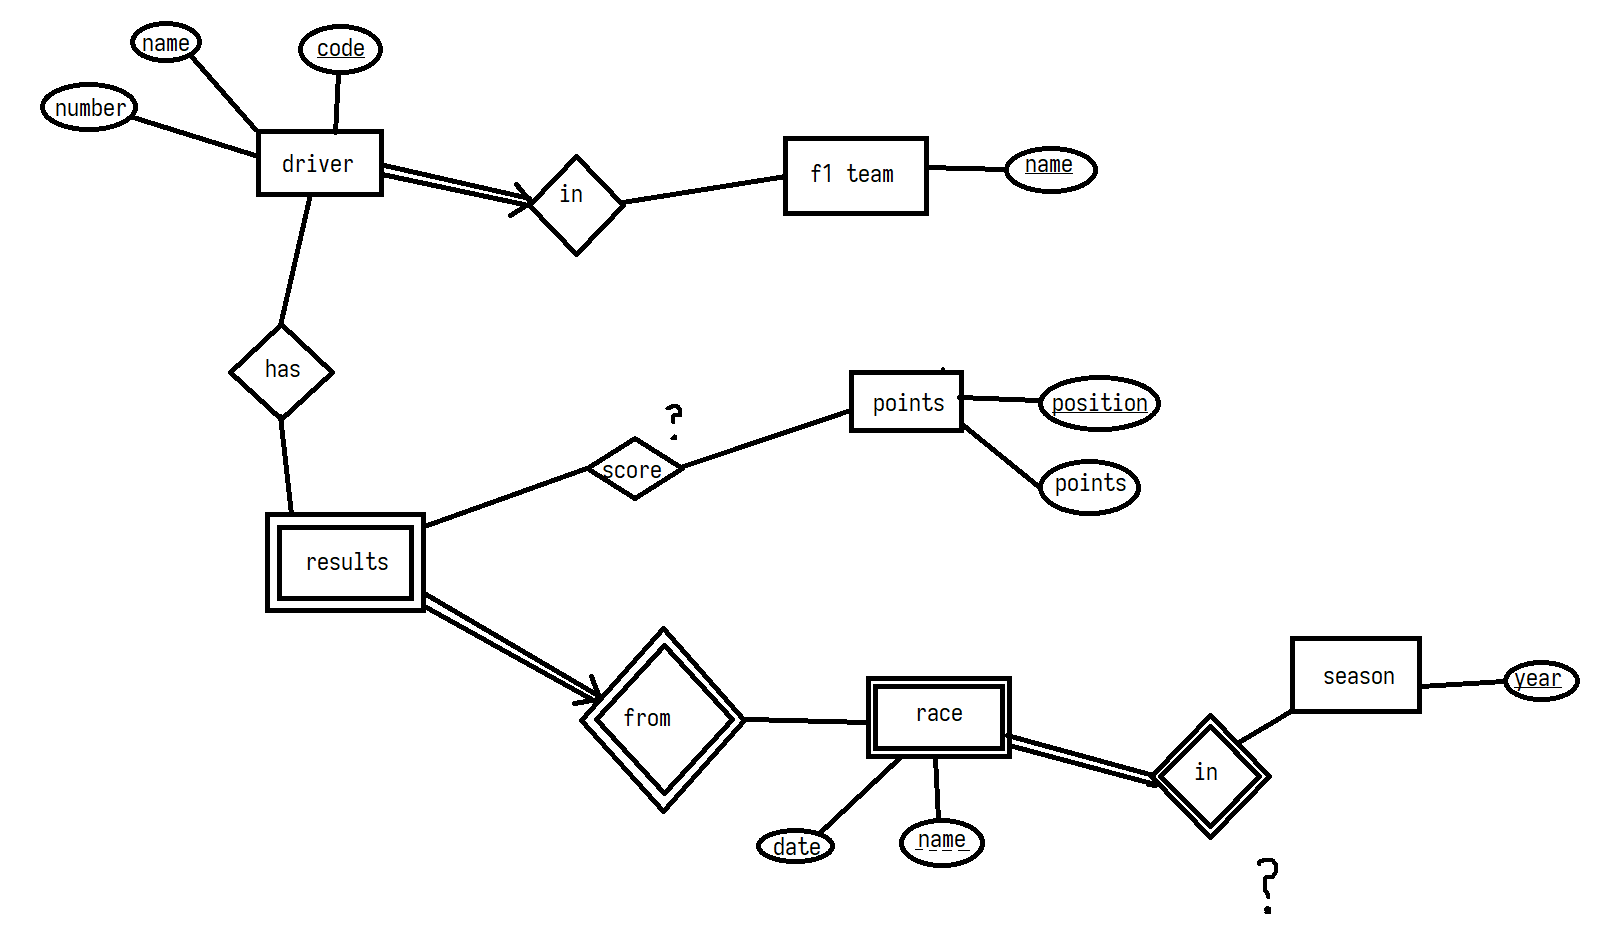
\includegraphics[scale=0.27]{f1_ER_diagram.png}
\end{figure}

There are two things that I am uncertain about with this diagram (note
where the question marks are):
\begin{enumerate}[label=(\arabic*)]
    \item Points are awarded to each driver determined by the results of
    the race (i.e., the position in which they finish). However, it
    makes sense to have the ``points'' table be separate, because the
    number of points a driver receives depends on their position (e.g.,
    first place always receives 25 points). I wasn't sure what the
    proper Chen notation was to connect the points table to the results
    table (my confusion arose from the fact that the position is
    determined by where the driver finishes, and I didn't know if the
    points table should bridge to the driver table, the results table,
    or both).

    \item My second confusion arose from the proper notation with having
    a race in a season. As it currently stands, a race is owned by a
    season, the season having a primary key of ``year'', and the race
    using the ``year'' foreign key and the race ``name'' partial key as
    its primary key. Each season can have a race in it only once (e.g.,
    there can be only one Italian Grand Prix in the 2022 season), but a
    race can appear in multiple seasons (e.g., the Italian Grand Prix
    also took place in the 2021 season, 2020 season, and so on). I
    wasn't sure what the proper notation for this would be.
\end{enumerate}

\section{Other Notes}

By my count, my ER diagram comes out to 8 tables.


\end{document}
